%************************************************
\chapter{Assessment of current Business Process Management Solutions}\label{ch:assessment}
%************************************************

The lack of flexibility in handling event subscription in business processes has been outlined in the previous chapters, and a set of additional requirements \textit{R1} to \textit{R3} for process management solutions have been presented.
In this section, we take a closer look at the capabilities of current solutions with regards to the event occurrence scenarios~(see~\autoref{ch:ps:eos}) to get a better understanding of the issues that arise when working with event subscription in business processes.

The assessment will be carried out on the basis of the \ac{BPMN} and Camunda, a state-of-the art and widely adopted business process engine~(\autoref{ch:bg:bpms}). Both tools shall be used \textit{as they are}, that means without utilizing their comprehensive extension mechanisms.
The main goal is to identify and illustrate the shortcomings of the current process technology stack by attempting to implement the requirements identified previously.
We therefor first investigate options to handle the \acs{EOS}s on the BPMN model level~(\autoref{ch:ass:models}) and then proceed to implementing early event subscription and event buffering in a set of Camunda processes~(\autoref{ch:assessment-implementation}).

Finally, the findings are discussed in \autoref{ch:ass:discussion} which leads to the presentation of three additional requirements, \textit{R4} to \textit{R6}.
The extended requirements will be referenced in \autoref{ch:flexibleeventsubscription} to develop a more refined subscription handling model.

\todo[inline]{which functionality should be evaluated exactly?: all occurrence scenarios, but no buffer policies. The buffer will always store the last version of the event and also deliver that version.}

\section{BPMN Models in presence of the Event Occurrence Scenarios}\label{ch:ass:models}

According the BPMN specification, the listening for an event starts only when the event element is enabled. The start of the listening is interpreted as the time of event subscription.
The motivating examples illustrate that process executions can be delayed or even blocked because of a late time of event subscription~(\autoref{ch:motivatingexamples}).
The subscription-time is put in relation to the time of event occurrence by the help of the event occurrence scenarios.

In this section, I first describe for each \ac{EOS} how a basic event implementation behaves in presence of the given scenario.
I then evaluate if it is possible to create a BPMN model that is free from unnecessary delay in these situations.
The investigations are carried out on the basis of the abstract process model shown in \autoref{fig:abstract-process-with-event}.
It uses an intermediate message catch event which follows an arbitrary process flow, represented through a collapsed sub-process.
The process terminates after the event is received.
It is assumed, that the event can occur independently from the preceding subprocess and therefor in accordance with any of the event occurrence scenarios. That enables us to investigate each EOS using this simple model.
The event behavior is comparable with the \textit{Eurotunnel Delay Event} considered in \textit{Example~1.1}\,. Depending on the discussed EOS, the motivating examples will be used for further illustration of the situations.


\begin{figure}[]
	\myfloatalign
	{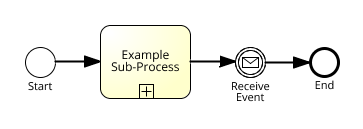
\includegraphics[width=0.7\linewidth]{chapters/assessment/generic-process-with-interm-event.png}}
	\caption{Generic process terminating after an intermediate message catch event}\label{fig:abstract-process-with-event}
\end{figure}


\subsection*{EOS1: The event occurs while the catch element is enabled}

The first scenario represents the case that is assumed by the BPMN 2.0 specification: 
The event occurs after the event element has been enabled and before it has terminated. It will be consumed by the catch event and the process flow can proceed without unnecessary delay.
In this scenario, the use of a simple intermediate catch event is sufficient.

\todo[inline]{Notably, there always is a certain delay when consuming an event through an intermediate catch event. The BPMN specification itself states that \textit{the handling consists of waiting for the Event to occur}.
However, that delay can theoretically be infinitely small. <-- maybe mention this at the beginning of 'problem statement' to differentiate between normal delay and unnecessary delay?}

\subsection*{EOS2: The event does not occur}

\begin{figure}[bth]
	\myfloatalign
	\subfloat[Parallel timer event]
	{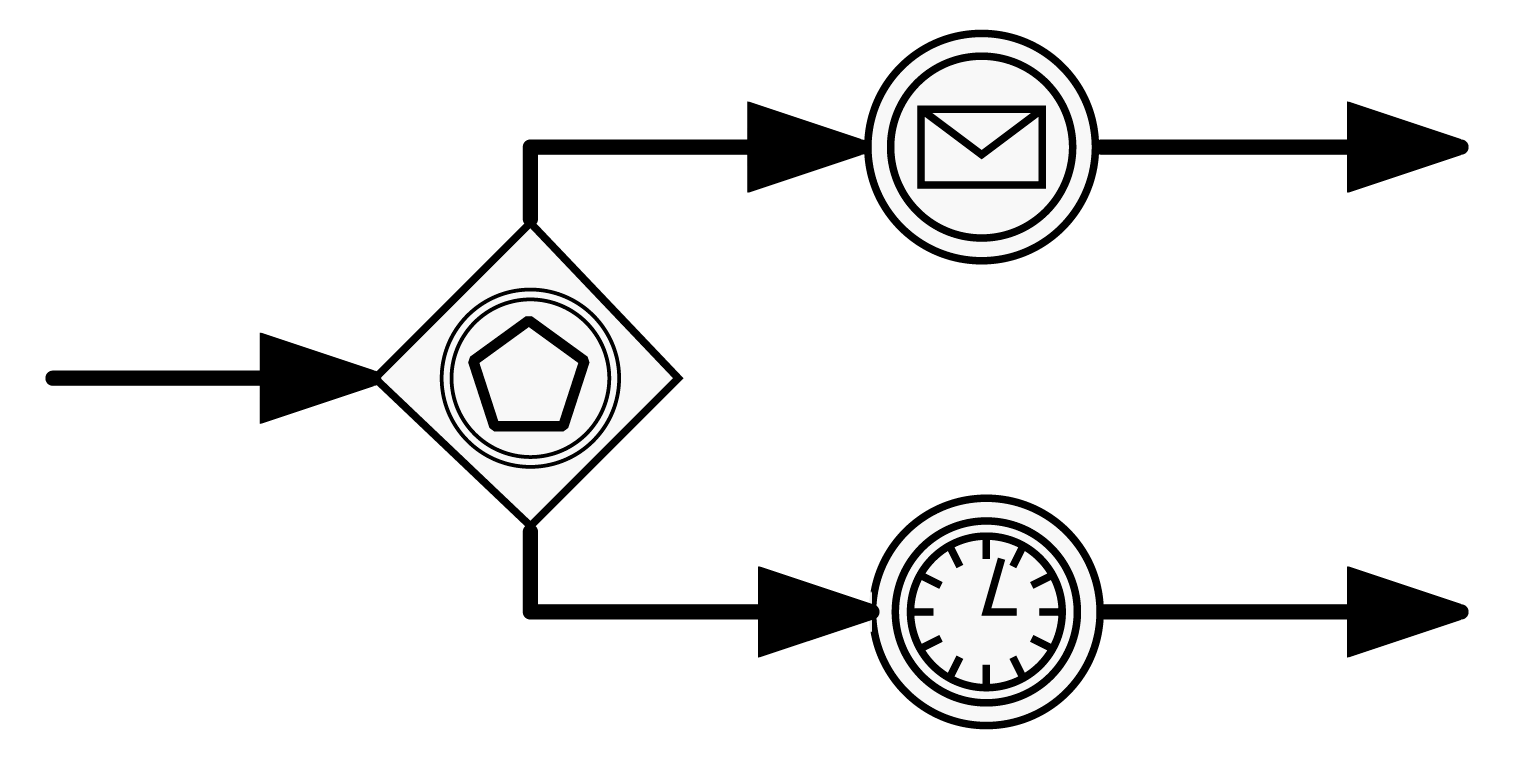
\includegraphics[width=.45\linewidth]{chapters/assessment/parallel-timer-event.png}} \quad
	\subfloat[Boundary timer event]
	{%\label{fig:example-b}%
		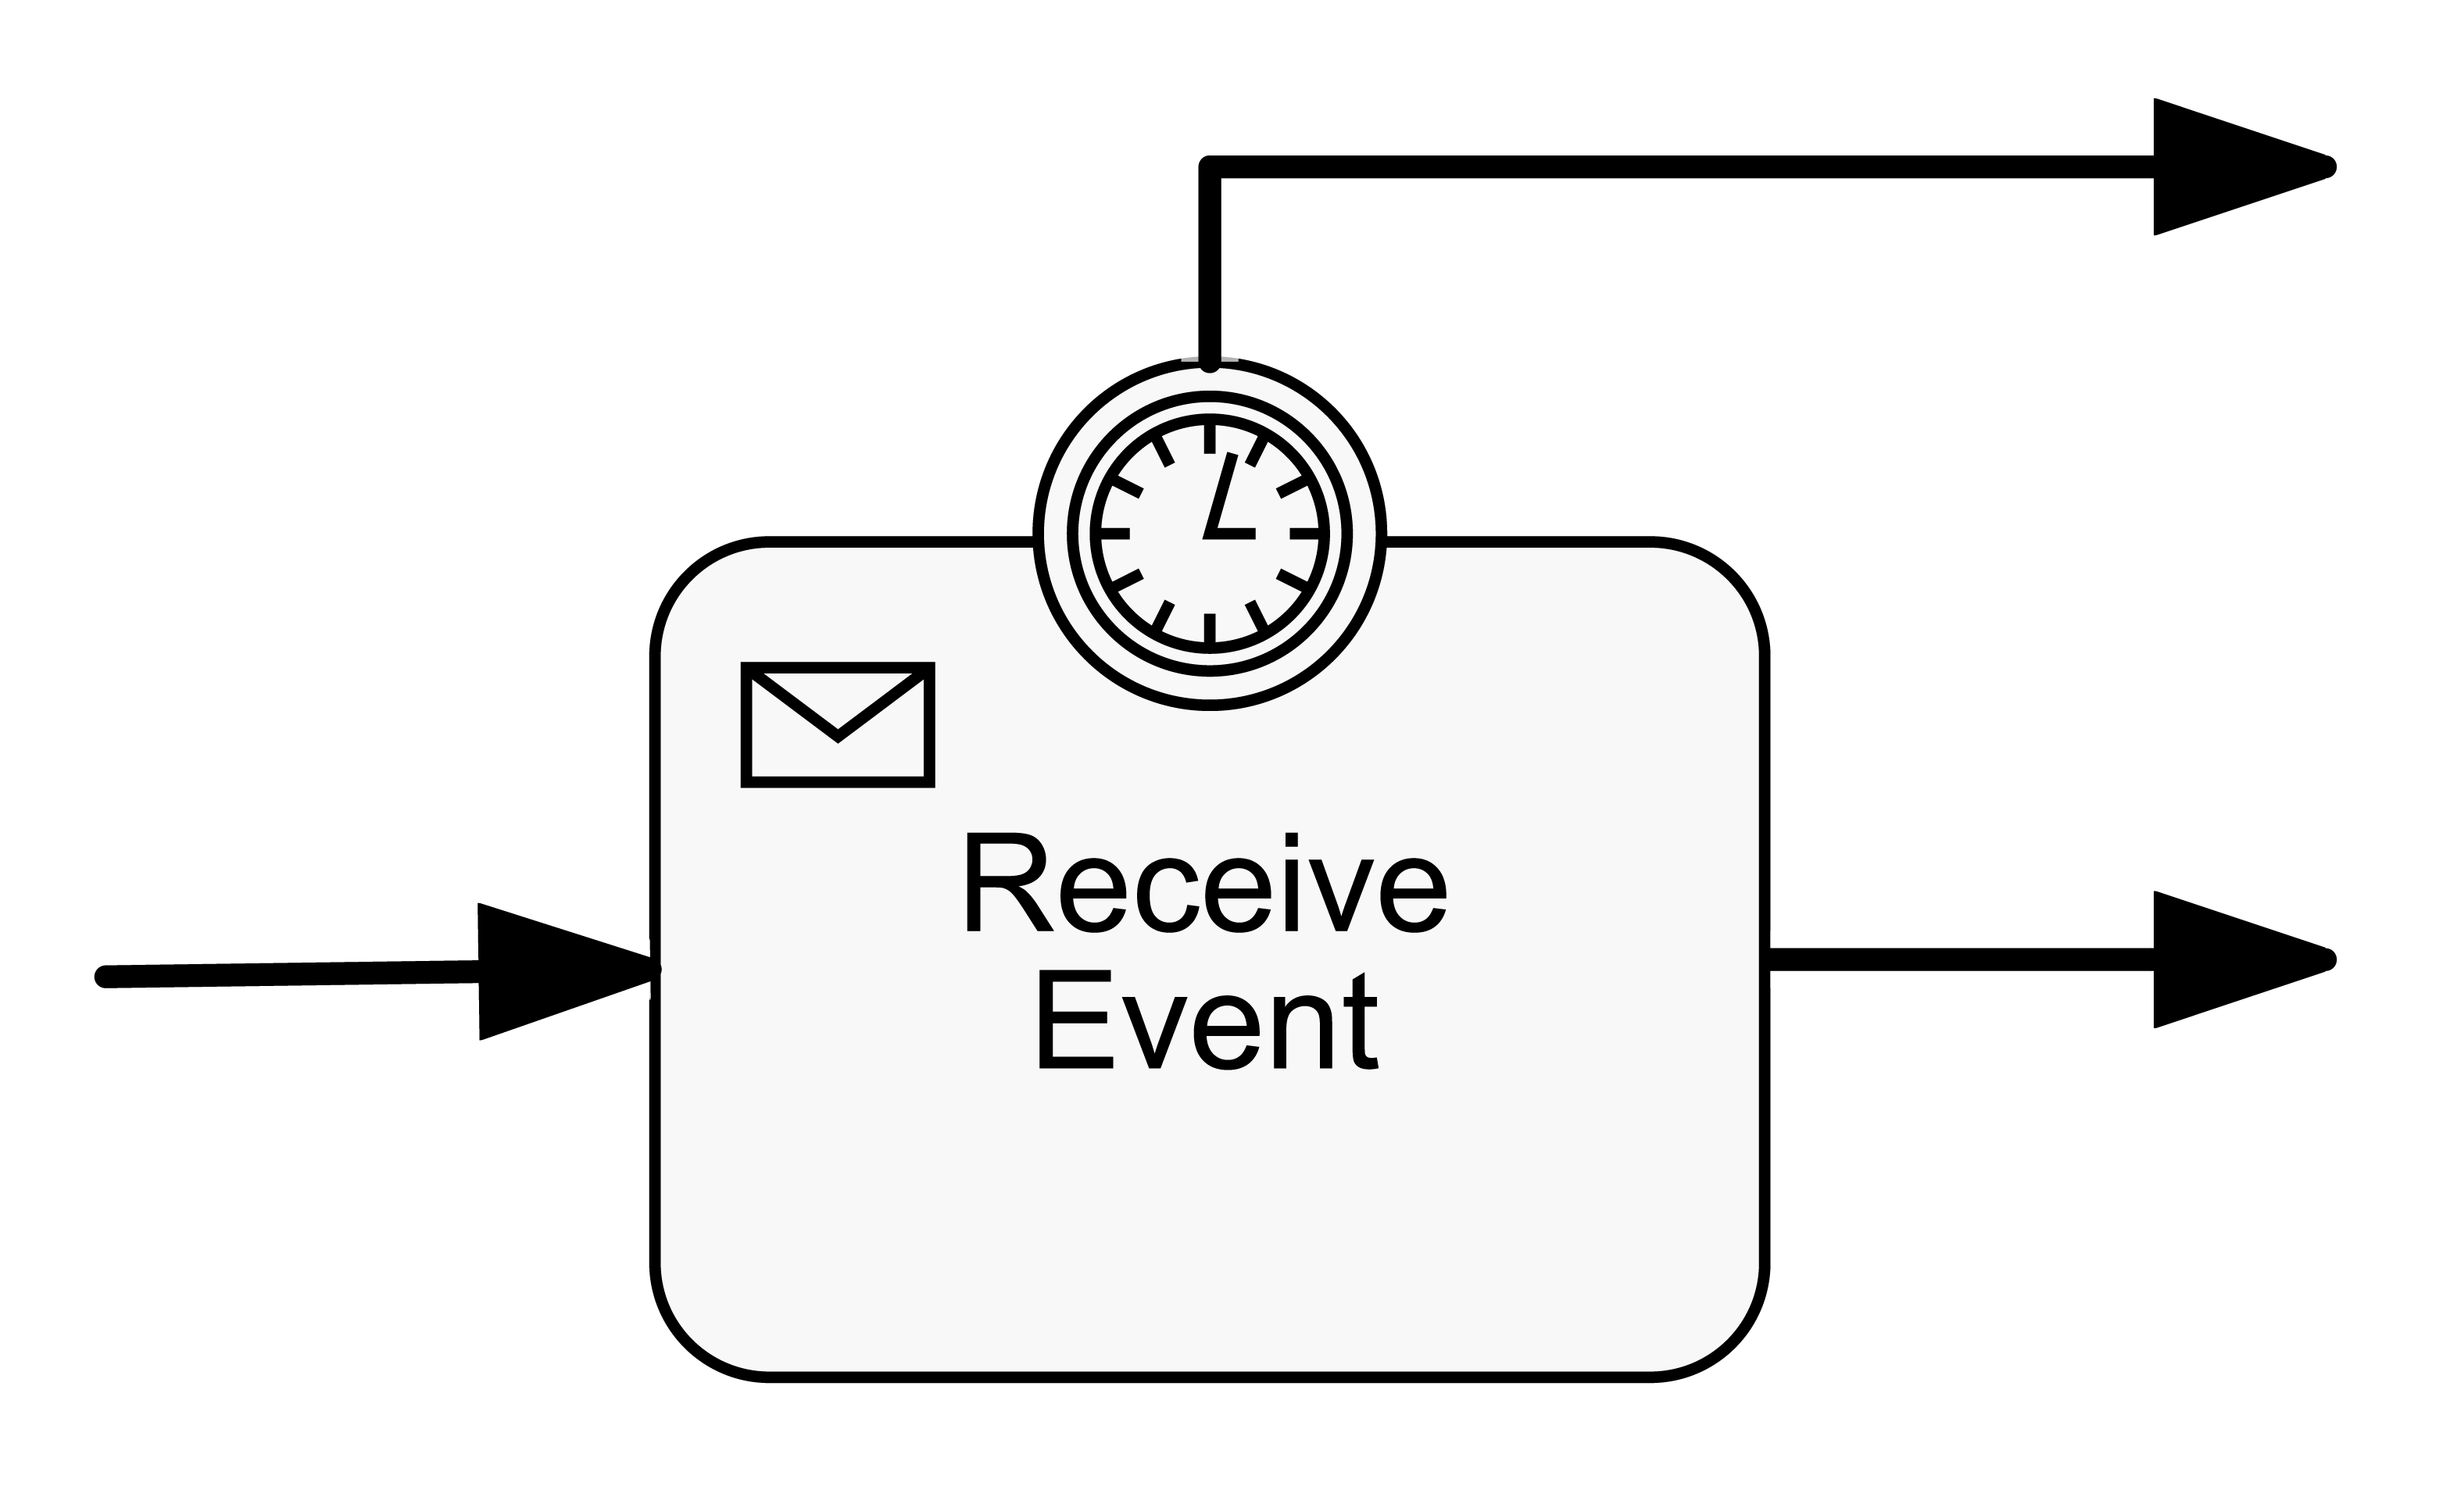
\includegraphics[width=.45\linewidth]{chapters/assessment/boundary-timer-event.png}}
	\caption[Tu duo titulo debitas latente]{Receipt of an intermediate message event, either interrupted by a~boundary event\,(a) or parallel timer event\,(b).}
	\label{fig:excerpt-event-with-timer}
\end{figure}

In certain situations an event might not occur at all. Given a basic event implementation like in \autoref{fig:abstract-process-with-event}, the process flow will get to a halt once it reaches the intermediate catch event and will not be able to proceed. While, depending on the process design, this might be the desired behavior, in many situations this is not acceptable.
In \textit{Example~1.2}, the process relies on the \textit{final arrival time} information from the customer. If the event does not occur, for example due to a mistake in a factory work-flow, the process execution waits for the event indefinitely.
To improve the process design, the logistics company decides that after waiting for the event for 30~minutes, an arbitrary delivery window shall be assumed. The waiting for the event shall be terminated so that the goods can be delivered immediately.

\autoref{fig:excerpt-event-with-timer} shows how this behavior can be implemented in two ways: (a)~By the help of an event-based gateway which puts a timer event in parallel to the intermediate catch event: If the timer event occurs before the message event is consumed, the message event is terminated immediately and the process flow proceeds from the timer event.
An alternative solution with equivalent semantics is depicted in~(b), using a receive task and an interrupting boundary timer event. Once the timer event fires, the receive activity is canceled and the process continues along the outgoing flow of the time event.
Any of the two model improvements will make sure that a process does not run into a lock if the expected event does not occur.


\subsection*{EOS3: Occurrence between Process instantiation and the enabling of the BPMN event}
\begin{figure}[]
	\myfloatalign
	{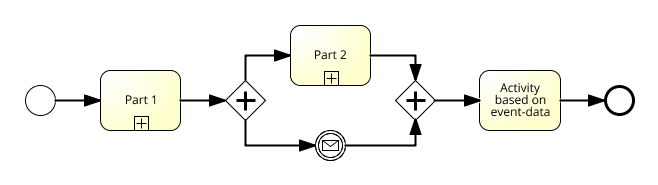
\includegraphics[width=1\linewidth]{chapters/assessment/parallel-gateway-early-subscription.png}}
	\caption{Event Element in parallel process flow}\label{fig:excerpt-parallel-gateway-event}
\end{figure}

In case the event occurs during process execution, but before the BPMN event element is enabled and thus listening for events, the occurrence will not be available for consumption. 
The execution will come to a halt at the event element as if the event did not happen at all.

\todo[inline]{could exemplify this at ex1.2, In the previously mentioned \textit{Example~1.2}}

To avoid a lock in this scenario, the intermediate catch event can be placed in parallel to the rest of the process flow using a parallel gateway. 
This is illustrated in \autoref{fig:excerpt-parallel-gateway-event}. The time of subscription to the event can be controlled by the position of the parallel split: To implement an event subscription right after process instantiation, the Parallel Gateway has to be the first element after the Start Event~(that means \textit{Part~1} in the illustration is empty). 
To implement the event subscription at a specific point during process execution, part of the process must execute before reaching the Parallel Gateway. As modeled in \autoref{fig:excerpt-parallel-gateway-event}, the event may occur at any time during the execution of the collapsed sub-process \textit{Part~2}. 

\subsection*{EOS4 and EOS5: Before Process Instantiation}\label{ass:model:buffered}
\begin{figure}[]
	\myfloatalign
	{\hspace*{-0.0cm}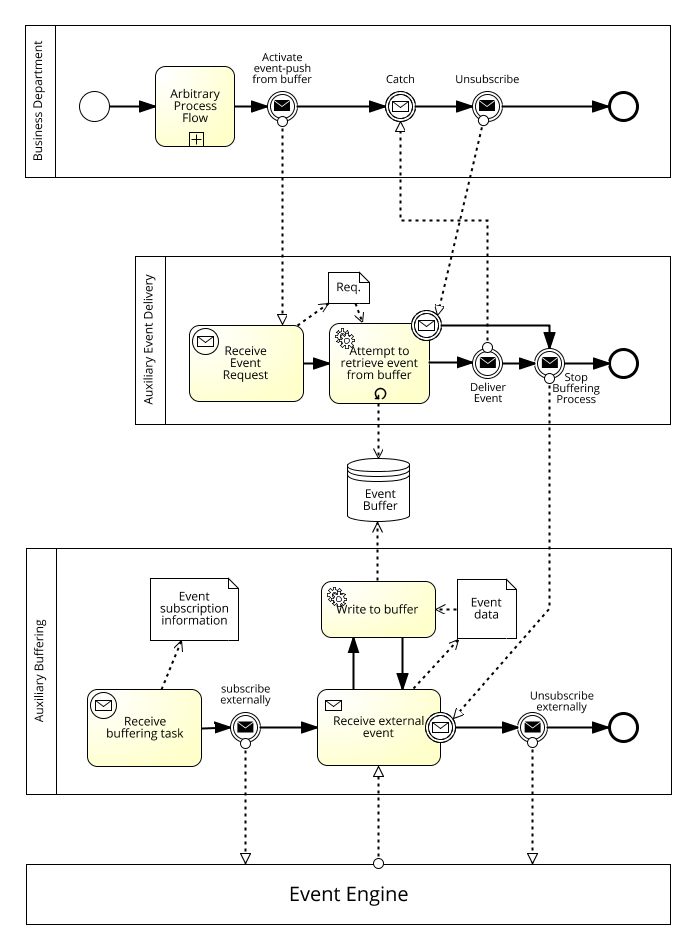
\includegraphics[width=1.2\linewidth]{chapters/assessment/2A_buffer_pushing.png}}
	\caption{Event Buffering through an auxiliary buffering process}\label{fig:aux-buffering-process}
\end{figure}

%intro
Any Events that happen before process instantiation will not be considered in a standard intermediate catch event. That applies to both scenarios, the occurrence between deployment and instantiation~(\textit{EOS4}) and an occurrence time before the deployment of the process in the Process Engine~(\textit{EOS5}).

%new elements
To create a process model that allows to catch an event before the process instance exists, three new elements are introduced in addition to the existing process referred to as \textit{target-} or \textit{original process}. The elements are: (1)~An additional \textit{Auxiliary Buffering Process} that can catch an incoming event independently from the target process; (2)~an \textit{Event~Buffer}, a temporary data-store that keeps event data until it is ready for consumption; (3)~an \textit{Auxiliary Event Delivery Process}, that retrieves events from the buffer and makes them available to the target process.
By introducing an additional process for listening to the event, the subscription time to the \textit{Event Engine} can be before instantiation or even deployment of the original process.
\autoref{fig:aux-buffering-process} shows the interaction of the original process, the two auxiliary processes and the data-store.

%how does that work in detail
%Auxiliary buffering
\paragraph{The execution flow}
To start listening for an event, the auxiliary buffering process has to be instantiated through a message start event containing the information necessary for the event subscription. 
The process subscribes to the event engine through a throwing event. It then waits for an event to occur in a receive activity \textit{Receive external event} and outputs the received event data to a DataObject. That object is then written to a persistent, global data-store \textit{Event Buffer} by the service task \textit{Write to buffer}. 
The design is able to handle multiple event occurrences, because, after writing to the buffer, the receiving activity is executed again. The buffering process terminates only once the \textit{Unsubscribe} event is received.
The implementation of the service task decides about the exact semantics of the buffering and hence about requirement~\textit{R3.3}. For the sake of simplicity, it is assumed that the buffer can hold a maximum of 1~element~(\textit{Size~Policy}) and the service task overwrites that element whenever a new one is available, specifying the retrieval order~(R3.3.4).
An implementation of the \textit{Lifetime Policy} is not provided. 
The consumption behavior~(\textit{R3.3.2}) is defined by the service task of the auxiliary delivery process: After the retrieval of an event from the buffer it remains available.

%original process and event delivery
After the buffering process is running, the original process can be instantiated. 
In the presented model, its intermediate catch event has been explicitly split into three events to fulfill the publish/subscribe paradigm: An initial send event to request events, a catch event to receive and a final send event to signal that no events shall be received anymore.
The initial send event instantiates the \textit{Auxiliary Event Delivery Process}, which tries to read from the event buffer and delivers the event to the original process if there is one available. 
The central looping activity will retry reading from the buffer until data becomes available and will only be terminated once the \textit{Unsubscribe}-event occurs.

%conclusions
\paragraph{Conclusions}
Thanks to the complex interaction of the three processes, the original process can consume the desired event, even though the event occurs before process instantiation. Consequently, \textit{EOS4}~can be handled by the model. 
Moreover, the \textit{Auxiliary Buffering Process} is not bound to a specific event, it works generically with any event information that is passed to it. For that reason it is also not bound to a specific process deployment and can buffer events even before a process has been deployed, so it handles scenario~\textit{EOS5}.
The buffering process can alternatively be started using an explicit message send event during process execution, similar to the \textit{Explicit Subscription Task} introduced in \cite{mandal:2017}. By that means, \textit{EOS1}~and \textit{EOS3} are also supported, which results in the fulfillment of requirement~\textit{R2.2}.

%BUT
It remains to be highlighted that this approach will only work for \textit{EOS4} and \textit{EOS5} if the buffering process is instantiated before the associated event occurs. As there are no other systems in place to automatically instantiate the process, it must be assumed that the process is manually started for each event and each process model that requires an early event subscription.
Furthermore, the number of processes running in the execution environment increases significantly. An instance of the buffering process is required for each event element that ought to make use of an event subscription time before deployment. For each instance of the original process and each buffered event, an instance of the auxiliary event delivery process must be started.
That puts additional load on the process engine which can endanger the reliability of business-critical processes and makes the management of processes and their instances more complex.
The downsides of the presented approaches are discussed in more detail in \autoref{ch:ass:discussion}.

\todo[inline]{Do I want to work with the requirements or not???}


\section{Implemention of Early Event Subscription using standard Camunda}\label{ch:assessment-implementation}
The previous chapter has shown that it is possible to create BPMN models to match each of the Event Occurrence Scenarios, though for the scenarios \textit{EOS4} and \textit{EOS5} the solution becomes increasingly complex.
In the next step I investigate the capabilities of Camunda as an example for a state-of-the-art business process engine.
Camunda shall be used without any code customization, that means as offered through the deployment package.
The solution presented in \autoref{ass:model:buffered} (\textit{EOS4} and \textit{EOS5}) has proven capable enough to handle all event occurrence scenarios, it is therefor the goal to implement a prototypical solution in Camunda in strong accordance with the BPMN model shown in \autoref{fig:aux-buffering-process}.

Two generic sample processes have been modeled for evaluate the functionality of the system. \autoref{fig:camunda-example-o3} shows a simple process with an explicit subscription activity to represent the listening to the event after process instantiation but before reaching the Catch Event (Scenario~\textit{EOS3}). It follows a sample activity that takes 15 seconds (implemented using a \textit{Script~Task}), the intermediate catch event and another script task that displays the content of the received message.
The example for scenarios \textit{EOS4} and \textit{EOS5}~(\autoref{fig:camunda-example-o4-o5}) comprises the following elements: After the start event follows an intermediate catch event, then an activity that prints the message of the event to console and last the process end event. Both figures show screen captures from the Camunda Modeler.

\begin{figure}[]
	\myfloatalign
	{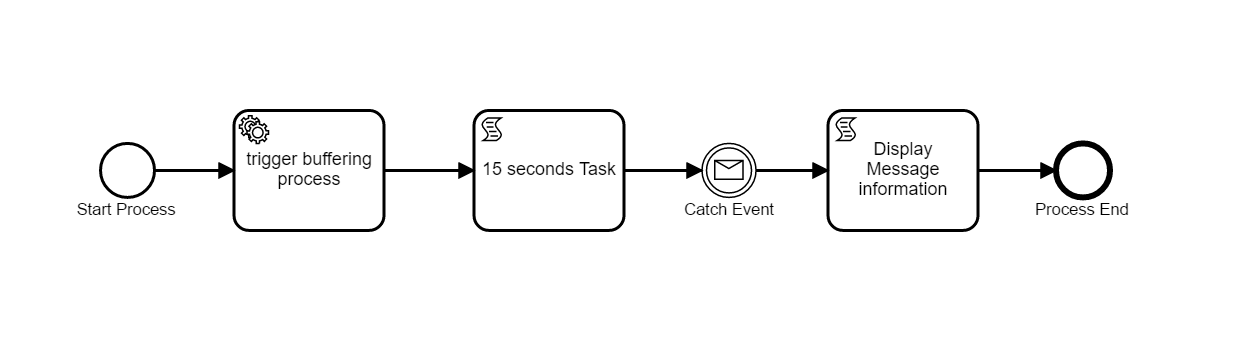
\includegraphics[width=1\linewidth]{chapters/assessment/example-o3.PNG}}
	\caption{Generic Example Process in Camunda for Occurrence Scenario \textit{EOS3}}\label{fig:camunda-example-o3}
\end{figure}

\begin{figure}[]
	\myfloatalign
	{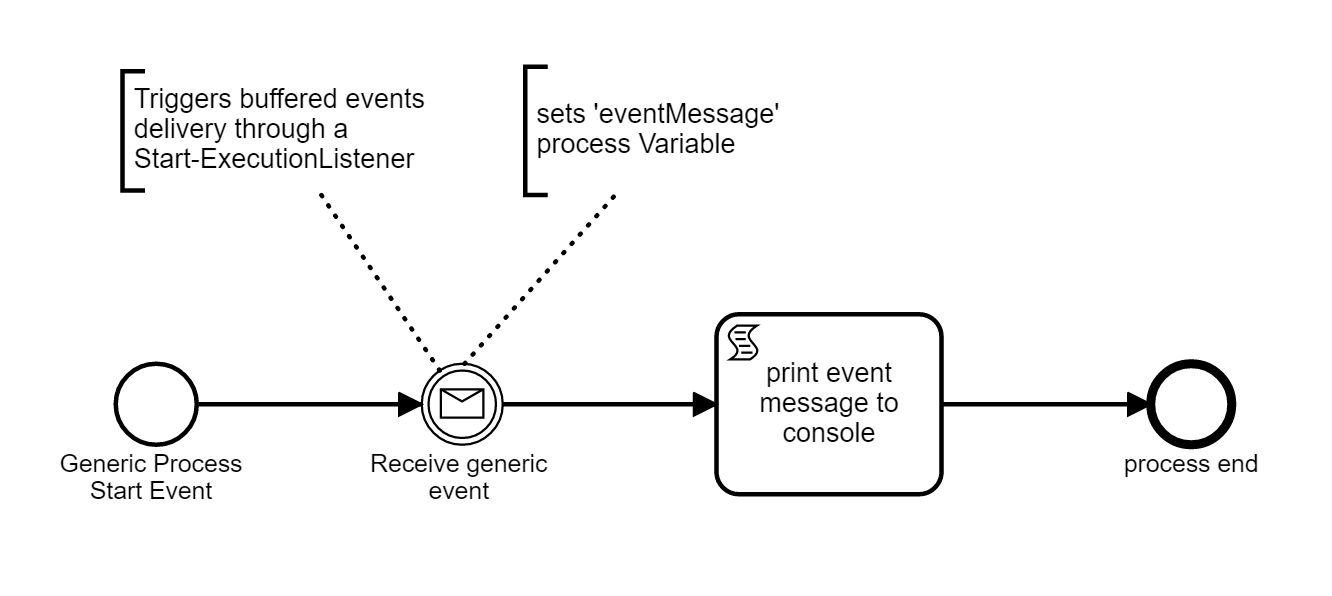
\includegraphics[width=1\linewidth]{chapters/assessment/example-o4-o5.PNG}}
	\caption{Generic Example Process in Camunda for Occurrence Scenarios \textit{EOS4} and \textit{EOS5}}\label{fig:camunda-example-o4-o5}
\end{figure}

\paragraph{Auxiliary Buffering Process}
The task of this process is to subscribe to a CEP Platform using a provided event query and start listening for events. Any incoming event must be stored in a data-store (\textit{Event Buffer}).
A local MySQL database has been chosen for persisting the event data because it is freely available, easy to set up, offers standardized access via SQL queries and Java connectors.
As complex event processing functionality itself is not required to demonstrate the use-case, the role of the \textit{Event Engine} is taken by a basic web-service which was specifically implemented in Python. It exposes a \textit{subscribe} method via \acs{HTTP} and can be used to trigger event messages associated to registered subscriptions.

\autoref{fig:camunda-aux-buffering-process} shows the final Buffering Process modeled in the Camunda Process Modeler. The process can be instantiated by issuing a \textit{Buffering Task} message. This message must contain three data fields: \textit{processDefinitionId}, to know which process definition the buffered messages belong to; \textit{messageName}, the name of the message event within the process; \textit{query}, the event query in the Esper Query Language.
Camunda will make the message data automatically available in the process instance as process variables, so they can be used during the execution of the Buffering Process.
After instantiation, the process reaches the activity \textit{Subscribe to Event Source}, a \textit{Java Service Task} that executes a HTTP call to the event engine. That call registers the event query in the platform, providing the process instance identifier and the message name. Based on this information, Camunda can correlate received events back to a specific process instance and message element.
After the subscription, the process reaches the receiving activity \textit{Wait for unsubscribe event} that will terminate the process as soon as the \textit{Unsubscribe} event has been received.
As long as this activity is active, events can be received through the attached non-interrupting boundary event. Incoming events have a field \textit{eventBody}, which contains the event information and becomes available through a process variable with the same name.
The boundary event triggers the service task \textit{Write eventBody to datastore}, which takes the data from the process variable and writes it to the MySQL Database (\textit{Global Event Buffer}).

%Notably, the Camunda process model appears less complex than the one presented in \autoref{ass:model:buffered} while still implementing the same functionality.

\begin{figure}[]
	\myfloatalign
	{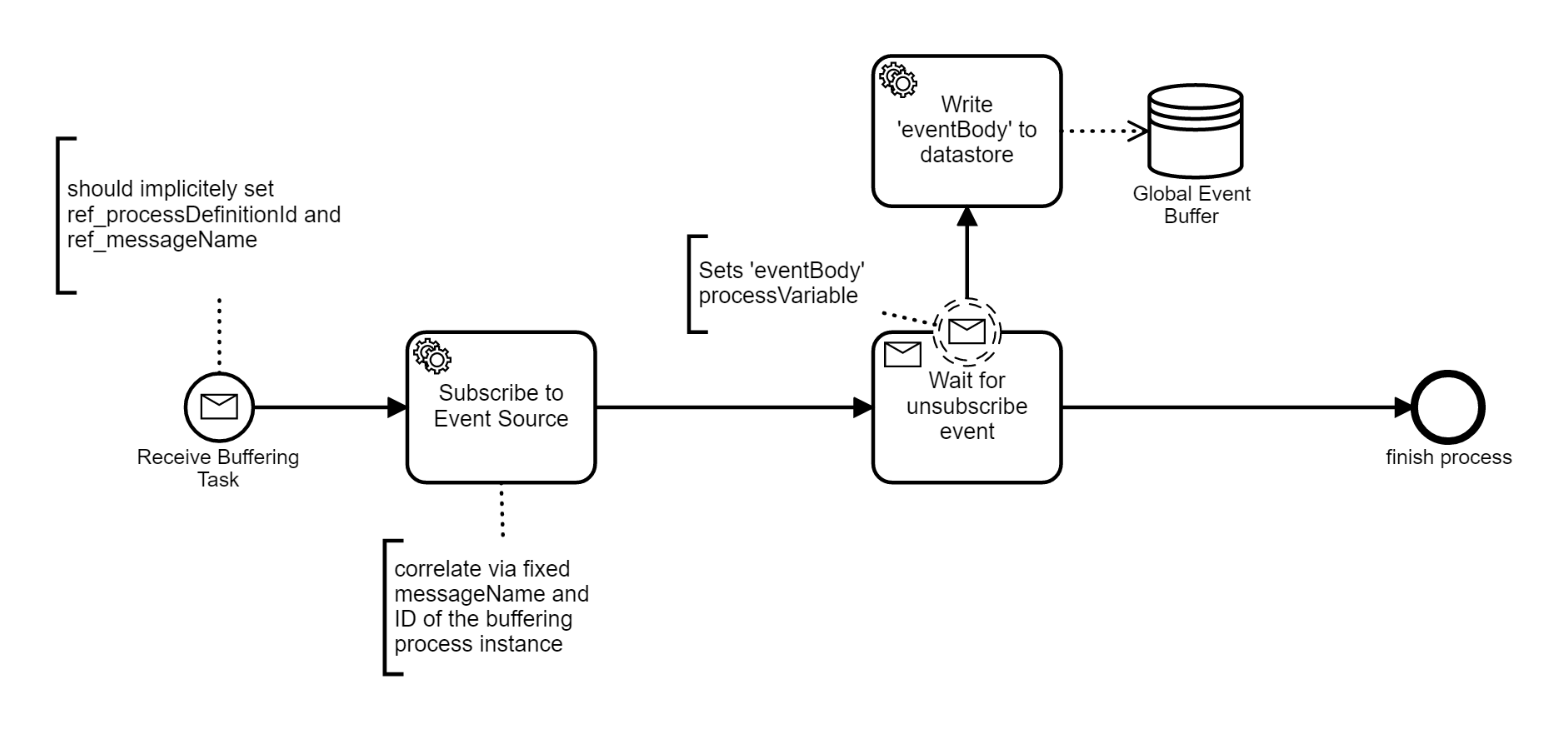
\includegraphics[width=1\linewidth]{chapters/assessment/buffering-process.PNG}}
	\caption{Auxiliary Buffering Process in the Camunda Modeler}\label{fig:camunda-aux-buffering-process}
\end{figure}

\paragraph{Auxiliary Event Delivery Process}
The delivery process (see \autoref{fig:camunda-aux-event-delivery}) reads the latest data from the buffer and sends it to the process instance. It can be started with a message that contains the \textit{processInstanceId} and the \textit{processDefinitionId} of the requesting process and the \textit{messageName} of the message event that is requested from the buffer.
A timer event \textit{Delay Timer} has been inserted to make sure that the requesting process is already listening for an event, when the delivery process sends the message. The outgoing execution flow is treated asynchronously.
It follows the service task \textit{Retrieve event from buffer}, which executes Java code to read from the MySQL Database \textit{Event Buffer} and store the event information in a process variable named \textit{eventMessage}.
The content of that process variable is sent to the original process in the send event, afterwards the execution is finished.

\begin{figure}[]
	\myfloatalign
	{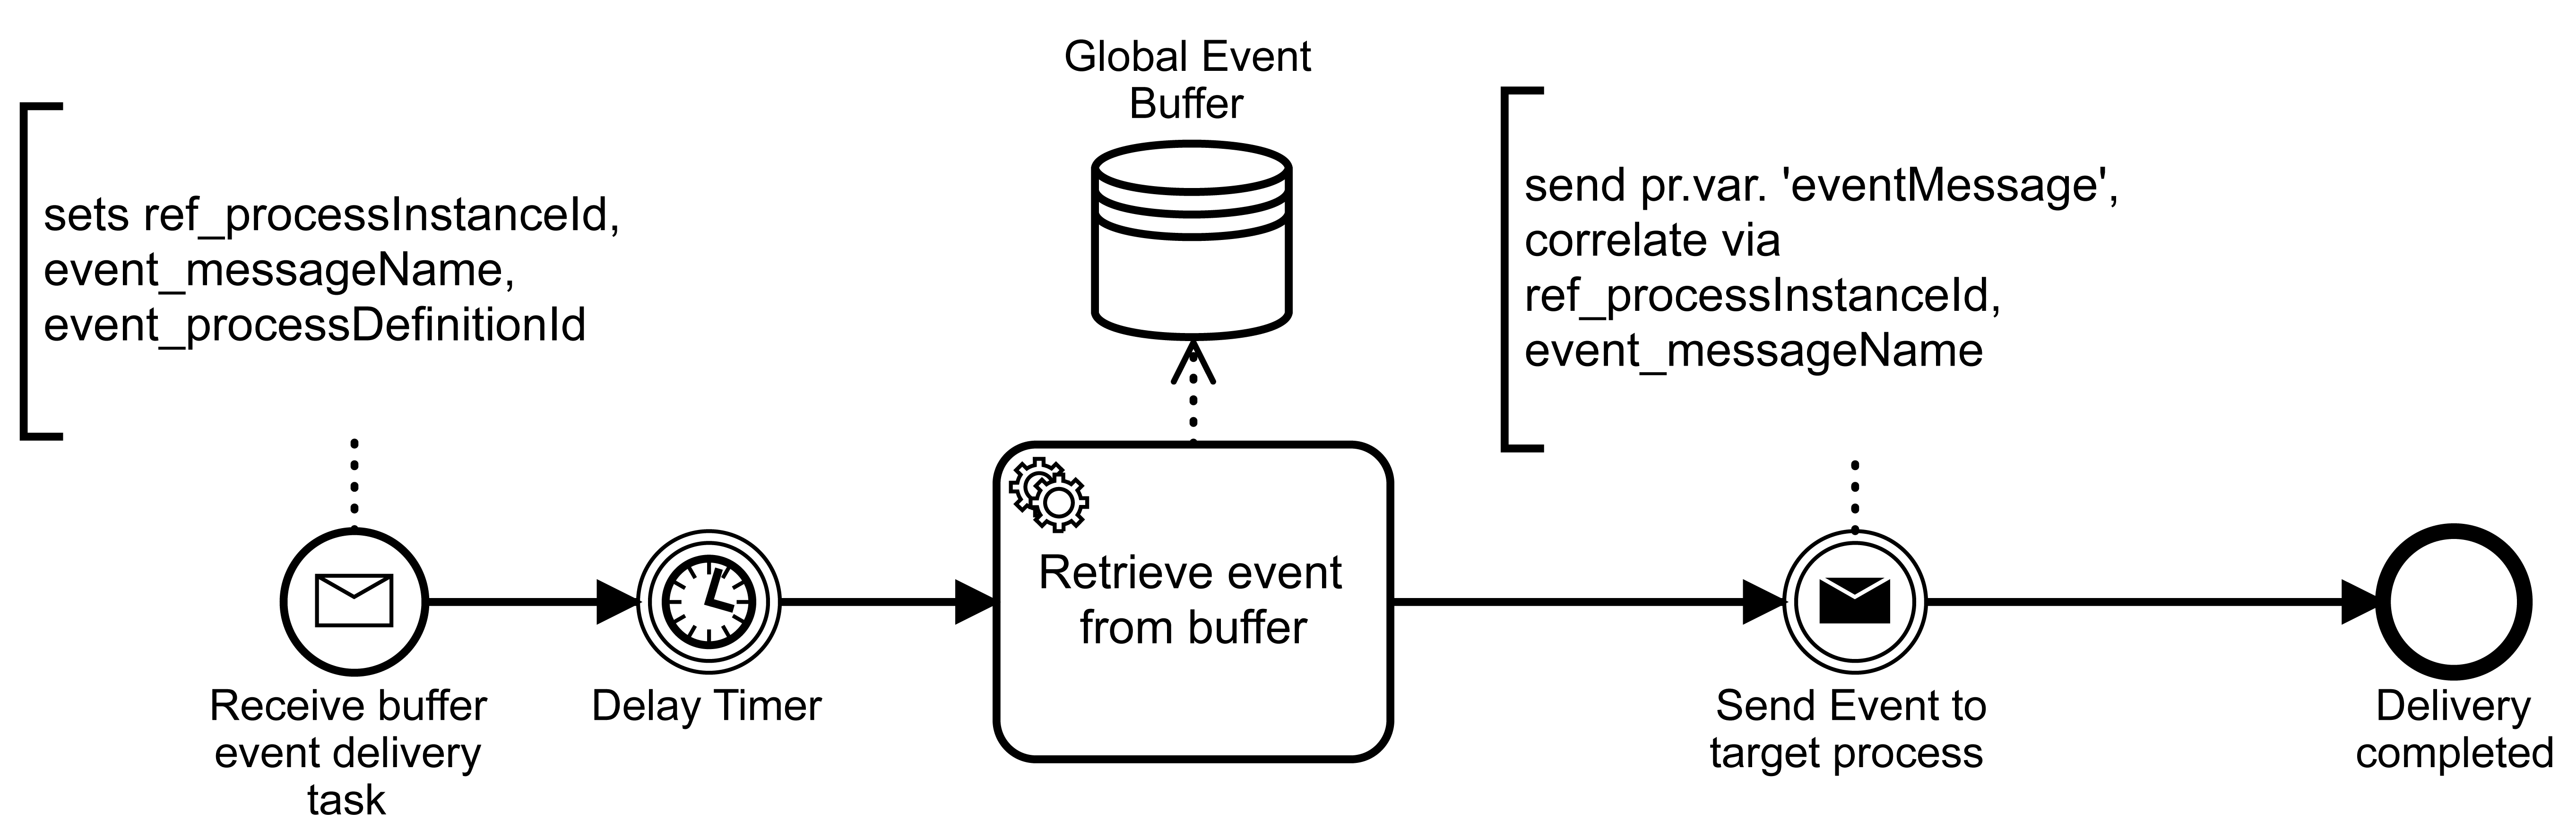
\includegraphics[width=1\linewidth]{chapters/assessment/buffer-delivery-process.PNG}}
	\caption{Auxiliary Event Delivery Process in Camunda Modeler}\label{fig:camunda-aux-event-delivery}
\end{figure}


\paragraph{Interaction of the Processes}
%In this implementation of flexible event subscription, the action of subscribing to the event source and the reception of events in the Original Process are splitted into two separate parts, each supported by an auxiliary process.
To initiate the subscription at the event source, the Auxiliary Event Buffering process has to be started.
For scenario \textit{EOS3}, this happens through an extra activity (\textit{Trigger Buffering Process}) during process execution, so that events after process instantiation are received by the Buffering Process.
In scenarios \textit{EOS4} and \textit{EOS5}, the subscription and thus the instantiation of the Buffering Process must happen before the instantiation of the Target Process. As there is no such mechanism in the standard Camunda Process Engine, the Buffering Process must be started manually, providing the \textit{processDefinitionId}, the \textit{messageName} and the \textit{eventQuery}.

Now that the \textit{Buffering Process} is running, any events matching the query will be stored to the buffer.
When the Target Process reaches the Catch Event, a request for buffered events is sent as a message to trigger the \textit{Auxiliary Event Delivery Process}.
This message is sent using a short piece of Java code that gets executed when the Catch Event is reached. 
The code is invoked by a Start ExecutionListener attached to the Catch Event. ExecutionListeners are offered by Camunda to execute own Java programs before or after relevant events during process execution, like the execution of an element in the process.
While the Original Process will now start listening for the desired events, the Event Delivery Process will send the buffered events as messages to the Original Process.

If no events have been received yet, all the involved processes remain active: the Buffering Process will keep listening for an external event. The Delivery Process will send an event to the Original Process as soon as there is one in the buffer. The Catch Event in the Original Process will keep listening for an Event.
The necessary communication for the termination of the processes and the unsubscribe-operation have not been implemented in this prototypical implementation, as they would not add particular value to the evaluation.

\paragraph{Conclusion}
The described implementation of the BPMN buffering concept presented in \autoref{ass:model:buffered} serves as a brief evaluation of the model. As illustrated by the help of the two examples, the resulting set of process applications allows to issue an event subscription flexibly according to the event occurrence scenarios.
While a thorough analysis was not the target of this section, it still provides an introduction to the capabilities of the Camunda process engine, which will take an important role again in \ref{ch:implementation}.

\todo[inline]{where is the code?}

Note that this is an investigative implementation that matches exactly the given use-case and is not meant to be used in production. It is neither flexible nor robust enough for that purpose, but suits very well in understanding the capabilities and the shortcomings of BPMN and Camunda when it comes to handling the Event Occurrence Scenarios.


\section{Discussion}\label{ch:ass:discussion}
The goal of this chapter was to get a better understanding of the capabilities of the tools when it comes to covering all event occurrence scenarios. 
Even though it has proven possible to implement a flexible event subscription time using standard BPMN 2.0 and Camunda, the success comes at a cost.
The downsides of the presented approach are presented in the following.

It was necessary to create two generic auxiliary processes for event buffering, to connect to a MySQL data-store and use ExecutionListeners to execute custom Java code in Camunda to cover all scenarios, \textit{O1} to \textit{O5}.

\todo[inline]{give them short names for reference? Or make one of them Requirement 5}


\paragraph{Missing automatic subscription handling\newline}

In the presented process models, separate process elements had to be added to handle event subscription and initiate event delivery. 
That conflicts with requirement \textit{R2}, which states that the subscription and un-subscription must be automatically handled by the process engine.
For the scenarios \textit{O4} and \textit{O5} the Buffering Process has to be triggered manually, because it must be executed before the target process is running. Camunda does not handle external event subscription itself, especially not before the process is running.

\paragraph{Additional model complexity\newline}

As additional process elements have to be added to handle event subscription and delivery, the models become more complicated and are less concentrated on the business case.
\todo[inline]{there could be a requirement that states that there should be no additional process elements unless there is an explicit subscription time}

\paragraph{Buffering is an IT Task\newline}

The auxiliary processes are not business tasks and are thus not suited to be modeled in BPMN.
Desired functionality can be put into Camunda BPMN models thanks to its flexibility to use Java code in Service Tasks or Event Listeners, but naturally the full functionality of the Event Buffer cannot be expressed using BPMN.
\todo[inline]{what exactly is the issue here?}

\paragraph{Added load on the Process Engine\newline}

Because of the aux processes, two additional processes have to be deployed in the process engine and are potentially running in parallel to any given process instance. For each Event Element used in a process the engine has to run an instance of the Buffering Process and, eventually, an instance of the Buffer Delivery Process.
That puts additional load on the process engine, which might prevent business critical processes from executing delay-free.

Even when the number of deployed and running auxiliary processes can be reduced through further optimizations there remains an event-management overhead as every event has to be handled twice: once when it is stored in the buffer and once when it's delivered to the target process.

\paragraph{Hidden Performance Limitations of the Process Engine\newline}

Given the large amount and high frequency in that events can occur in reality, optimal performance is required for an event-buffering module.
Running essential parts of the buffering within the process engine might pose performance limitations that cannot be influenced without tempering with the process engine code.

\medskip \noindent
\todo[inline]{write connector to next chapter: it has been shown that... therefor we do ...}


\section{Requirements extension}\label{ch:ass:reqextension}
\begin{description}
	\item[R2 Automatic Subscription Handling:] 
	The subscription to event sources is handled implicitly by the process execution environment based on the modeled subscription information as required by \textit{R1} and \textit{R2}. Similarly, the removal of a subscription is performed as soon as a subscription becomes unnecessary.	
\end{description}

+ model complexity
+ no influence on performance

